\documentclass[12pt,a4paper, oneside]{Thesis} 

%\usepackage[left=35mm,right=35mm,top=50mm,bottom=25mm]{geometry}

% The default font size and one-sided printing (no margin offsets)
%[12pt, oneside]
%packages

%counter
\newcounter{cap}

\newcounter{ref}

\usepackage{amsmath}
\usepackage{amsfonts}
\usepackage{amssymb}

\usepackage{array}

\usepackage[T1]{fontenc}
\usepackage[utf8]{inputenc}

\usepackage{times}
\usepackage[romanian]{babel}
\usepackage{combelow}
\usepackage{newunicodechar}
\usepackage{amsmath}
\usepackage{sidecap}
\usepackage{titlesec}

\hypersetup{linkcolor = black}

\usepackage[T1]{fontenc}
\usepackage{pgfplots}
\usepackage{leftidx}

\usepackage[T1]{fontenc}
\usepackage[utf8]{inputenc}
\usepackage{babel}
\usepackage[math]{blindtext}

\newunicodechar{Ș}{\cb{S}}
\newunicodechar{ș}{\cb{s}}
\newunicodechar{Ț}{\cb{T}}
\newunicodechar{ț}{\cb{t}}
\usepackage{hyperref}

\usepackage{hhline}
\usepackage{booktabs}

\usepackage{graphicx}

\newcommand\scalemath[2]{\scalebox{#1}{\mbox{\ensuremath{\displaystyle #2}}}}



\usepackage{amsmath}
\usepackage{hyperref}
\usepackage{multicol}

\usepackage{scrextend}

\usepackage{lipsum}
\usepackage{titlesec}
\usepackage{titletoc}

%settings
\usepackage{fancyhdr} 
\fancyhead{}%clear all headers
\fancyhf{}
\chead{}
\rhead{}
\renewcommand{\headrulewidth}{1pt}
\renewcommand{\footrulewidth}{1pt}
\cfoot{\thepage}
%\pagestyle{fancy} 
%\pagenumbering{gobble}
\setlength{\parskip}{0pt}

\usepackage{titlesec}
%\usepackage{lipsum}
\usepackage{listings}



\newcommand*{\SkipTocEntry}{\addtocontents{toc}{\gobblefour}}
%\usepackage{polyglossia}
%\usepackage{tocvsec2}

\newcommand*{\justifyheading}{\raggedleft}
\titleformat{\chapter}[display]
 % {\normalfont\bfseries\filcenter}{}{10em}{\large}
 {\normalfont\bfseries\filcenter}{}{}{\large}
  
\titleformat{\section}
  {\normalfont\sffamily\normalsize\bfseries}
  {\thesection}{0.2em}{}
 
 %commands
\newcommand{\mychapter}[2]{
    \setcounter{chapter}{#1}
    \setcounter{section}{0}
    \chapter*{#2}
    \addcontentsline{toc}{chapter}{#2}
}

%\renewcommand{\listfigurename}{List of plots}
%\usepackage{blindtext} 
%\renewcaptionname{romanian}{\contentsname}{cuu} 
  
%%\addtolength{\oddsidemargin}{-.875in}
%%\addtolength{\evensidemargin}{-.875in}
%%\addtolength{\textwidth}{1.75in}
%
%\addtolength{\topmargin}{25mm}
%\addtolength{\}{25mm}
%%\addtolength{\textheight}{1.75in}
%\usepackage[top=25.4mm, left=25.4mm, right=20mm, bottom=25.4mm, includehead,includefoot]{geometry}


%\usepackage[top=25.4mm, left=25.4mm, right=20mm, bottom=25.4mm,headsep=\baselineskip]{geometry}


%%page settings

\usepackage{geometry}
 \geometry{
 a4paper,
 total={210mm,297mm},
 left=20mm,
 right=20mm,
 top=20mm,
 bottom=20mm,
 }
 %\parindent=2cm;

\graphicspath{{Pictures/}} % Specifies the directory where pictures are stored

%\usepackage[square, numbers, comma, sort&compress]{natbib} % Use the natbib reference package - read up on this to edit the reference style; if you want text (e.g. Smith et al., 2012) for the in-text references (instead of numbers), remove 'numbers' 
%\hypersetup{urlcolor=blue, colorlinks=true} % Colors hyperlinks in blue - change to black if annoying
%\title{\ttitle} % Defines the thesis title - don't touch this

\makeglossaries
\newacronym{api}{API}{Application Programming Interface}
\newacronym{dll}{DLL}{Dynamic-link library}
\newacronym{xml}{XML}{Extensible Markup Language}
\newacronym{json}{JSON}{JavaScript Object Notation}
\newacronym{sql}{SQL}{Structured Query Language}
\newacronym{ip}{IP}{Internet Protocol}
\newacronym{tcp}{TCP}{Transmission Control Protocol}
\newacronym{ansi}{ANSI}{American National Standards Institute}

\begin{document}\thispagestyle{fancy}
%\frontmatter % Use roman page numbering style (i, ii, iii, iv...) for the pre-content pages

\titleformat*{\section}{\normalsize\bfseries}
\titleformat*{\subsection}{\normalsize\normalfont}
\titleformat*{\subsubsection}{\normalsize\normalfont}
\titleformat*{\paragraph}{\normalsize\bfseries}
\titleformat*{\subparagraph}{\normalsize\bfseries}

  
\pagestyle{fancy} % The page style headers have been "empty" all this time, now use the "fancy" headers as defined before to bring them back

\fancyhead[L]{\fontsize{10}{10}\selectfont\emph\bfseries\textcolor{black!70}{\textit{Facultatea de Inginerie Electrică şi Ştiinţa Calculatoarelor \\ Departamentul Automatică şi Tehnologia Informaţiei \\}}}

\fancyhead[R]{\fontsize{10}{10}\selectfont\emph\bfseries\textcolor{black!70}{\textit{Automatică şi Informatică Aplicată \\}}}

 % Begin numeric (1,2,3...) page numbering
\mainmatter

\label{Cuprins}
%\addcontentsline{toc}{chapter}{Cuprins}
\tableofcontents

%\addcontentsline{toc}{chapter}{Listă de figuri}
\listoffigures

\listoftables

\renewcommand*{\acronymname}{Listă de acronime}
\printglossaries


%----------------------------------------------------------------------------------------
%	THESIS CONTENT - CHAPTERS
%----------------------------------------------------------------------------------------



\pagestyle{fancy} % Return the page headers back to the "fancy" style

% Include the chapters of the thesis as separate files from the Chapters folder
% Uncomment the lines as you write the chapters

% abbreviations:


% Chapter 1
\stepcounter{cap}
%\chapter{cap1}
\label{cap1}

\mychapter{1}{Capitolul \arabic{cap} \\ INTRODUCERE}
%\chapter{\arabic{cap}.Introducere} % Main chapter title

\label{Chapter1} % For referencing the chapter elsewhere, use \ref{Chapter1} 

\thispagestyle{fancy}

%-----------------------------------------------------------------
 
\section{Tema de proiectare} 

\section{Stadiul actual al problemei abordate} 
În momentul actual există diverse companii precum Google, General Motors sau Volkswagen care dezvoltă propriile sale soluții de navigare predictivă.
\vspace{6pt}
\\Google furnizează alerte predictive de mai mult de 5 ani ca parte a funcționalității Google Now de pe dispozitivele Android.
\vspace{6pt}
\\La un atelier de inovare de la sfârșitul anului 2014, Volkswagen și-a prezentat la sediul său din Wolfsburg, Germania, propria sa soluție in-car de oferire de sugestii de rute alternative chiar și în cazul în care utilizatorii nu folosesc sistemul de navigație pentru o destinație uzuală. 
\vspace{6pt}
\\Alți producători de automobile, precum General Motors, au testat soluții pentru autovehiculele electrice de tip plug-in, cum ar fi modelul Chevrolet Volt, care va păstra automat alimentarea electrică pentru ultima porțiune a unei rute dacă destinație se află într-o zonă rezidențială, sau chiar să folosească o parte din bateria de rezervă pentru cazul în care sistemul prezice că autovehiculul va fi alimentat în curând.
\vspace{6pt}
\\Se poate spune deci, că fiecare producător preferă să-și dezvolte propriile soluții ce au un scop limitat și strict aplicat nevoilor lor, din motive clare de marketing și vânzare.

\section{Scopul şi obiectivele proiectului} 
Obiectivul principal este să se dezvolte un modul de navigare ce are ca scop estimarea rutelor posibile ale unui autovehicul.
\vspace{6pt}
\\Acest modul va fi împachetat sub forma unei biblioteci cu legare dinamică (\acrshort{dll} ) și va fi destinat utilizării de către orice aplicație de navigație.
\vspace{6pt}
\\Având ca scop obiectivul principal, s-au definit și câteva obiective intermediare:

\begin{itemize}
 \setlength\itemsep{0em}
	\item Deciderea asupra funcționalităților oferite de modul
	\item Deciderea asupra modului de stocare al datelor
	\item Împărțirea pe unității software de lucru
	\item Crearea diagramei de arhitectură
	\item Finalizarea scrierii codului
	\item Testarea modulului realizat
	\item Evindențierea posibilelor erori și oferirea de soluții
\end{itemize}

\section{Domeniul de aplicabilitate} 
Domeniul în care proiectul dezvoltat ar avea cea mai mare aplicabilitate este industria automobilistică, mai specific în cadrul aplicațiilor de navigare. În momentul de față acest domeniu este unul în plină ascensiune, tocmai de aceea se caută constant noi modalități  de a satisface nevoile utilizatorului, da a rezolva cerințele noi apărute, de a ușura condusul unui autovehicul și chiar de a face un pas înainte către dezvoltarea vehiculelor autonome.

\section{Structura pe capitole} 
	\begin{enumerate}
	 \setlength\itemsep{0em}
		\item Introducere\\
		Primul capitol începe cu o introducere în domeniul automobilisticii, prezentându-se câteva utilizări ale principiului și actualitatea sa în ziua de azi.
		
	    \item Baza de date\\
	    În acest capitol sunt prezentați factorii de decizie cu cea mai mare semnificație asupra tipului de date de baze ales. Totodată, capitolul 2 face și o scurtă introducere în cadrul SQLite pentru o mai bună înțelegere a scopului și structurii acesteia în cadrul proiectului.
	    
		\item Arhitectura software\\
		Capitolul 3 descrie structura software folosită în scopul dezvoltării algoritmului de predicție, explicând în detaliu legatura dintre unitățile software și rolul pe care acestea îl
îndeplinesc.

		\item Descrierea algoritmilor\\
		Acest capitol se axează pe logica din spatele funcțiilor principale îndeplinite de fiecare unitate software în parte.
		
		\item Gestionarea erorilor\\
		Scopul capitolului 5 este de a face cunoscute erorile ce sunt predispuse să apară în urma utilizării modulului de predicție, dar și a unor eventuale soluții.
		
		\item Concluzii și dezvoltări ulterioare\\
		Ultimul capitol al proiectului concluzionează dezvoltarea și rezultatele obținute. \\
		În urma realizării acestui proiect, a studierii necesităților și așteptărilor utilizatorului comun de la un sistem de navigație, dar și a analizei soluțiilor deja existente se prezintă posibile direcții de dezvoltare.
	\end{enumerate}
% Chapter 1
\stepcounter{cap}
%\chapter{cap1}
\label{cap2}

\mychapter{2}{Capitolul \arabic{cap} \\ BAZA DE DATE}
%\chapter{\arabic{cap}.Introducere} % Main chapter title

\label{Chapter2} % For referencing the chapter elsewhere, use \ref{Chapter1} 

\thispagestyle{fancy}

%-----------------------------------------------------------------
\section{Alegerea tipului de bază de date} 
	Nevoia modulului de a stoca şi de a accesa datele stocate anterior a dus la realizarea unui mic studiu în vederea alegerii tipului de bază de date cel mai potrivit.

	\subsection{Factori de decizie} 
	\begin{itemize}
	 \setlength\itemsep{0em}
		\item Consistenţa datelor stocate
		\item Utilizarea RAM-ului
		\item Timp de accesare la pornirea aplicaţiei
		\item Timp de accesare în cadrul aplicaţiei
		\item Spaţiul ocupat pe disc
		\item Compatibilitate cu versiunile anterioare
	\end{itemize}

	\subsection{Soluţii propuse}
	În următorul tabel, se presupune ca pentru fişierele binare, XML şi JSON este necesară încărcarea datelor la pornirea aplicaţiei. SQLite oferă însă soluţii de căutare inteligente, nefiind necesară încărcarea tuturor datelor la pornirea aplicaţiei.

	\begin{table}
	\caption{Compararea principalelor metode de stocare a datelor pe baza factorilor de influenţare}
	\resizebox{\textwidth}{!}{\begin{tabular}{ | c | c | c | c | c |}
	\hline
		& \textbf{Binar} & \textbf{XML sau JSON} & \textbf{SQLite} & \textbf{Memorare în Cloud} \\ 
	\hline
	 Consistenţa datelor stocate & Nu & Nu & Da & Da \\
	\hline
	 Utilizarea RAM-ului & Ridicat & Scăzut & Mediu & Mediu \\
	\hline
	 Timp de accesare la pornirea aplicaţiei & Mediu & Ridicat & Scăzut & Scăzut \\
	\hline
	 Timp de accesare în cadrul aplicaţiei & Scăzut & Scăzut & Mediu & Ridicat \\
	\hline
	 Spaţiul ocupat pe disc & Scăzut & Ridicat & Scăzut & Foarte scăzut \\
	\hline
	 Compatibilitate cu versiunile anterioare & Nu & Da & Da & Nu \\
	\hline
	\end{tabular}}
	\end{table}

	\subsection{Soluția aleasă}
	S-a decis folosirea SQLite ca format pentru baza de date deoarece îndeplinea toate criteriile specificate.


\section{Structura bazei de date}


\begin{figure}[h!]
  \centering
    \centering{%
      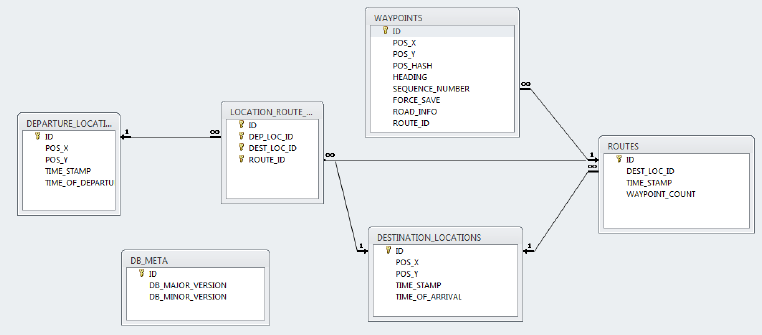
\includegraphics[width=0.9\textwidth]{Figures/baza_date.png}}
  \caption{Structura tabelelor de date şi relaţiile dintre ele}
\end{figure}

Tabelele din figura de mai sus sunt folosite pentru realiza structura întregii baze de date.
\vspace{6pt}
\\Tabela meta este folosită la identificarea versiunii bazei de date. Acest lucru este necesar pentru a detecta compatibilitatea şi pentru a permite migrarea către o versiune mai recentă. 
\vspace{6pt}
\\Datele înregistrate sunt separate în puncte de plecare, destinaţii, rute şi waypoint-uri. O rută este întotdeauna formată din mai multe waypoint-uri, unul sau mai multe puncte de plecare şi una sau mai multe destinaţii. Ruta (waypoint-urile) sunt stocate numai o singură dată, în timp ce toate punctele de plecare şi destinaţiile sunt stocate. În acest fel, numărul de destinaţii poate influenţa probabilitatea rutei.
\vspace{6pt}
\\Accesul la date se face prin SQLite. Toate datele stocate pot fi atât citite cât şi modificate.



% Chapter 1
\stepcounter{cap}
%\chapter{cap1}
\label{cap3}

\mychapter{3}{Capitolul \arabic{cap} \\ ARHITECTURA SOFTWARE}
%\chapter{\arabic{cap}.Introducere} % Main chapter title

\label{Chapter3} % For referencing the chapter elsewhere, use \ref{Chapter1} 

\thispagestyle{fancy}

%-----------------------------------------------------------------
În acest capitol este prezentată partea structurală a modulului cât şi unităţile software din care acesta este format.

\section{Limbajul C++}
Limbajul de programare C++ reprezintă de fapt o vastă colecție de comenzi folosite pentru controlul computerelor, numite și cod.
\vspace{6pt}
\\C++ este un limbaj de programare orientat pe obiecte ce a fost dezvoltat ca o extensie a originalului limbaj C în anul 1980. Este considerat a avea un nivel de dificultate intermediar, deoarece acoperă atât funcții de nivel înalt cât și de nivel scăzut.
\vspace{6pt}
\\Potrivit Fundației C++ Standard, limbajul oferă un sitem de memorie sistemică și un calcul structural ce seamănă foarte mult cu programarea celor mai multe computere. Acesta este folosit la o multitudine de sarcini, de la extragerea datelor din bazele de date la afișarea graficii jocurilor video sau chiar la controlarea dispozitivelor electronice atașate computerului.
\vspace{6pt}
\\Deoarece poate fi folosit pe orice sistem de operare, C++ este un limbaj de programare universal ce este găsit pe majoritatea computerelor.

\subsection{Obiectivele de proiectare}
C++ a fost inițial creat de Bjarne Stroustrup în cadrul Laboratoarelor AT\&T Bell, ca o cale de a depasi limitările limbajelor de programare deja existente, precum C și Simula.
\vspace{6pt}
\\C++ a fost creat cu scopul de a oferi flexibilitate, eficiență și o organizare structurală. În mod specific, mecanismele de încorporare abstractă au fost proiectate pentru a face față celor mai dificile și solicitante sarcini de programare.
\vspace{6pt}
\\C++ suportă abstractizarea datelor, programarea generică dar și programarea orientată pe obiecte. Deoarece c++ a fost gândit pentru a fi un limbaj de programare cu scop general, este foarte ușor de folosit și de utilizat.

\subsection{Funcționalitate multiplă}
C++ este foarte popular deoarece este extrem de funcțional. Este folosit pentru a crea sisteme de operare, drivere de dispozitiv și protocoale de rețea.
\vspace{6pt}
\\Este de asemenea utilizat pentru a dezvolta aplicații pentru baze de date, foi de calcul și procesare de text. Deoarece este un limbaj cu scop general, este potrivit pentru dezvoltarea oricărui tip de software. Acest lucru este posibil prin intermediul a peste 10 sisteme unice de implementare și sute de biblioteci, manuale și jurnale tehnice.
\vspace{6pt}
\\Deoarece C ++ permite programatorilor să creeze rapid programe în limite urgente de timp și spațiu, C ++ este ideal pentru manipulări hardware directe în constrângeri în timp real. Într-un astfel de cod, previzibilitatea performanței este cel puțin la fel de importantă ca și viteza brută.
\vspace{6pt}
\\Fiabilitatea C ++ a dus la favorizarea organizațiilor de tranzacționare, bancare, de asigurări, militare și de telecomunicații. 

\subsection{Avantaje}
C ++ este un limbaj foarte portabil, ceea ce înseamnă că programatorii pot scrie programe indiferent de limitele hardware și de sistemul de operare. Ca rezultat, programatorii pot dezvolta un program inițial care este tradus sistematic pe diferite platforme.
\vspace{6pt}
\\Orice program care a fost dezvoltat în limbajul original C poate fi ușor mutat în C ++ fără modificări majore. Deoarece C ++ oferă flexibilitate, programatorii sunt capabili să creeze construcții puternice și să introducă noi obiecte conceptuale și aplicații abstracte.
\vspace{6pt}
\\Ca rezultat, C ++ permite programatorilor să controleze și să manipuleze resursele hardware pentru a produce programe de funcționare înalte. C ++ vine cu câteva dezavantaje, cum ar fi numeroase erori de securitate și funcționalitate slabă a dezvoltării web.
\vspace{6pt}
\\Limbajul de programare C ++ este astfel unul din limbajele cele mai utilizate și versatile pe care toți începătorii ar trebui să-l învețe.

\section{Enterprise Architect} 
Sparx Systems Enterprise Architect este un instrument de modelare vizuală și de proiectare bazat pe OMG UML.
\vspace{6pt}
\\Platforma suportă: proiectarea și construirea de sisteme software, modelarea proceselor de afaceri, și modelarea domeniilor bazate pe industrie.
\vspace{6pt}
\\Este folosită de întreprinderi și de organizații nu numai pentru să modelarea arhitecturii sistemelor lor, ci și pentru a procesa implementarea acestor modele în întregul ciclu de viață al dezvoltării aplicațiilor.
\vspace{6pt}
\\Enterprise Architect este construit pe baza specificațiilor UML 2.
\vspace{6pt}
\\Utilizarea profilelor UML extinde capabilitățile de modelare iar validarea modelelor garantează integritatea.
\begin{figure}[h!]
  \centering
   \centering{%
   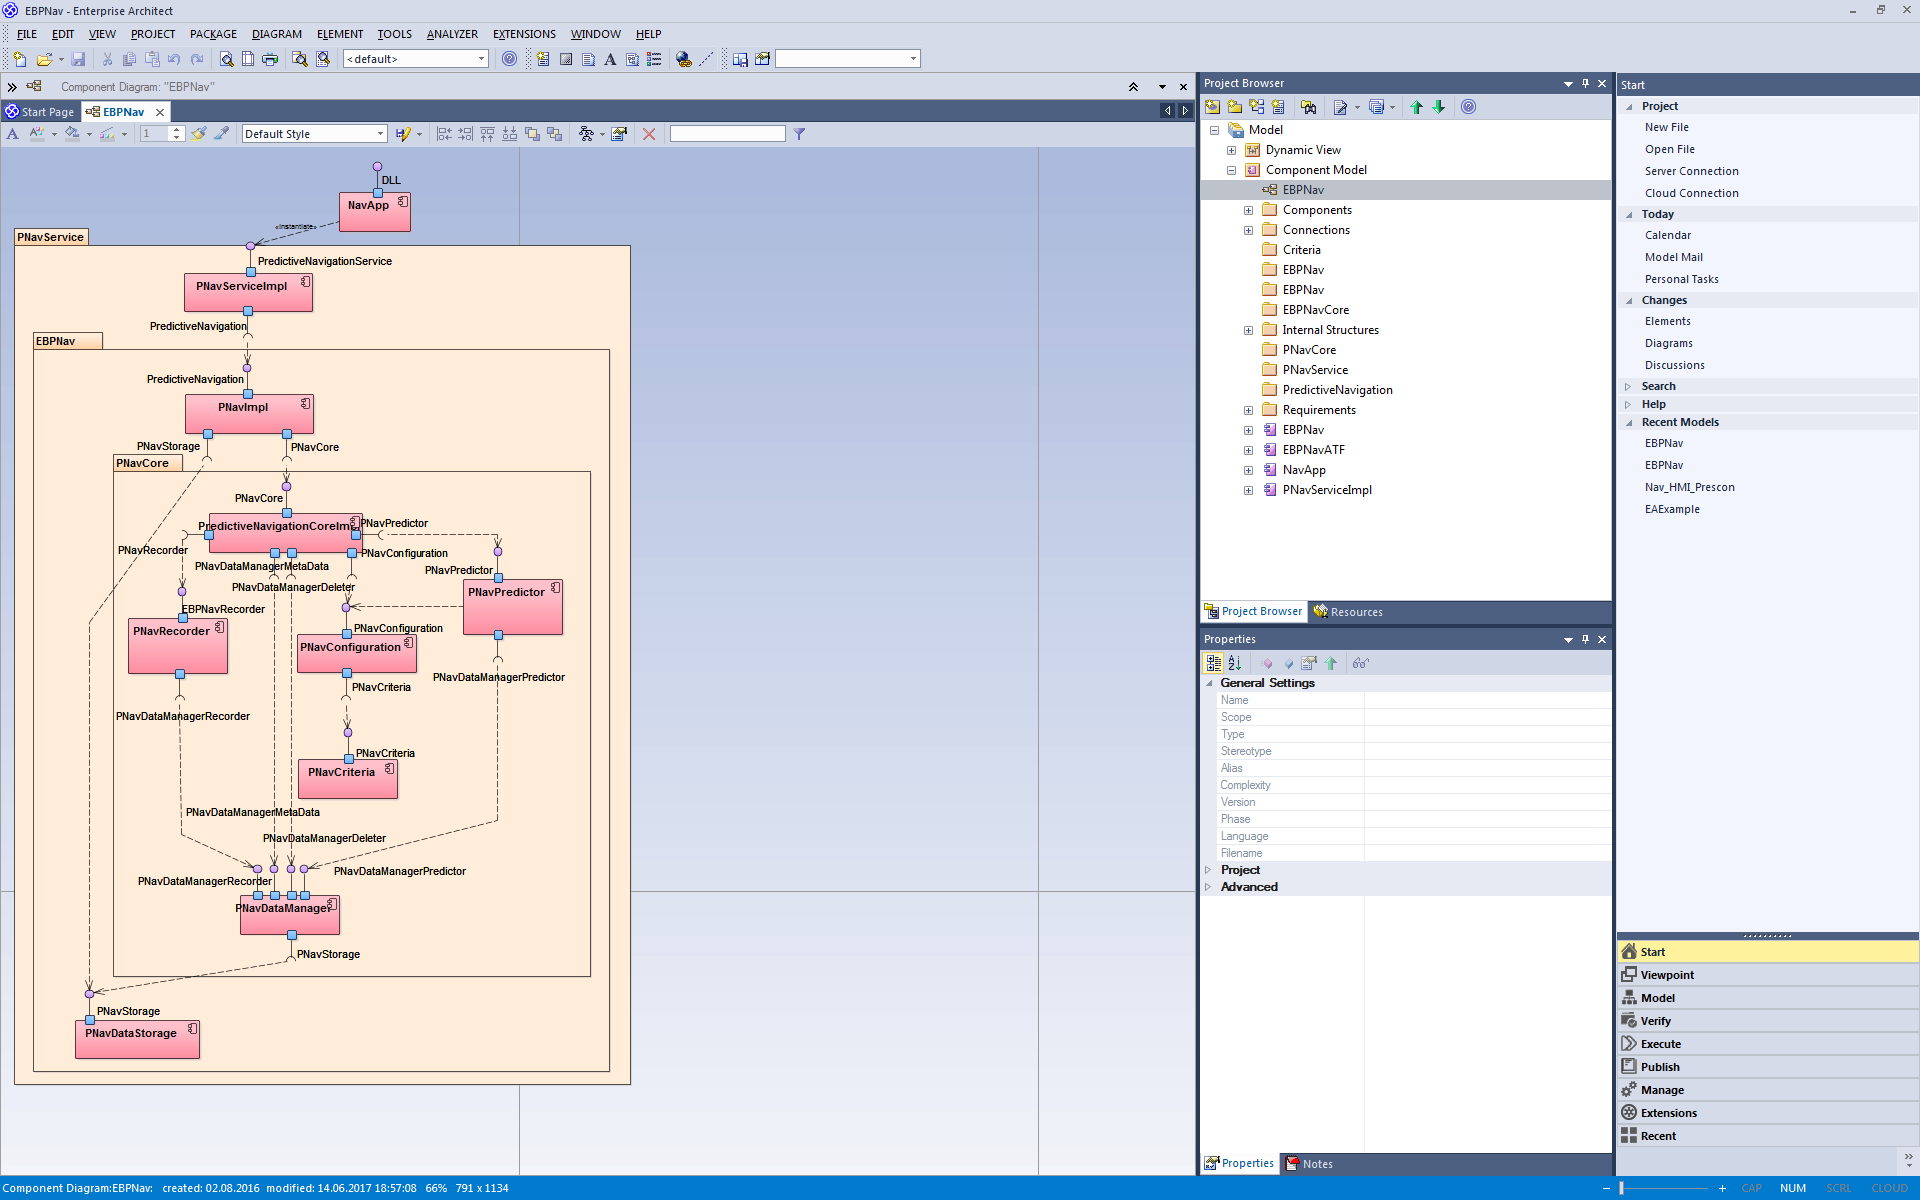
\includegraphics[width=0.9\textwidth]{Figures/ea.png}}
  \caption{Captură de ecran din Enterprise Architect}
  \end{figure}	

\subsection{Diagramele UML}
UML este o modalitate de vizualizare a unui program software folosind o colecție de diagrame.
\vspace{6pt}
\\Notația a evoluat de la munca lui Grady Booch, James Rumbaugh, Ivar Jacobson și Rational Software Corporation pentru a fi folosită pentru design orientat pe obiecte, dar de atunci a fost extinsă pentru a acoperi o varietate mai largă de proiecte de inginerie software. Astăzi, UML este acceptat de către Grupul de Management al Obiectului(OMG) ca standard pentru modelarea dezvoltării de software.
\vspace{6pt}
\\Termenul de UML vine de la Unified Modeling Language (limbaj unificat de modelare). UML 2.0 a ajutat la extinderea specificației UML originale pentru a acoperi o parte mai mare a eforturilor de dezvoltare software, inclusiv practicile Agile.
\vspace{6pt}
\\Deși este folosit în mod obișnuit în ingineria software, este un limbaj bogat care poate fi folosit pentru a modela structurile de aplicații, comportamentul și chiar procesele de afaceri. Există 14 tipuri de diagrame UML care vă ajută să modelați aceste comportamente, ele putând fi împărțite în două categorii principale; Diagrame structurale și diagrame comportamentale. 

	\begin{itemize}
	 \setlength\itemsep{0em}
		\item Diagramă tip clasă
		\item Diagramă tip componentă
		\item Diagramă de implementare
		\item Diagramă tip obiect	
		\item Diagramă tip pachet 
		\item Diagramă tip profil
		\item Diagramă tip structură compozită
		\item Diagramă tip scenariu
		\item Diagramă de activitate
		\item Diagramă tip stare mașină
		\item Diagramă de secvență
		\item Diagramă de comunicare
		\item Diagramă de interacțiune generală
		\item Diagramă de timp
	\end{itemize}


\begin{figure}[h!]
  \centering
   \centering{%
   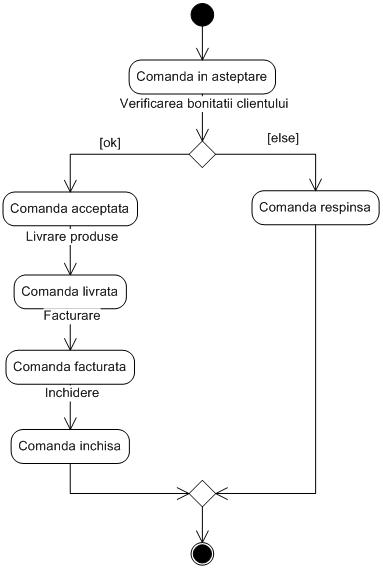
\includegraphics[width=0.5\textwidth]{Figures/diagrama_uml.jpg}}
  \caption{Diagramă de tip statechart pentru cazul realizării unei comenzi}
  \end{figure}	

\section{Deciderea asupra comportamentului sincron și asincron} 
	Fiecare mod de executare a operațiilor are propriile sale avantaje și dezavantaje.
	Există operaţii care ar putea necesita mai mult timp pentru a se termina de executat (>100ms) şi nu este direct vizibil faptul dacă acestea au fost declanşate de către o cerere (e.g. o  nouă poziţie este trimisă).
	\vspace{6pt}
    \\O cerere poate declanşată din fire de execuţie diferite.
	Există posibilitatea ca acest lucru sa fie realizat sincron, în afara modului, între cereri şi răspunsuri, fapt ce poate duce la deadlock.

	\subsection{Factori de decizie} 
	\begin{itemize}
	 \setlength\itemsep{0em}
		\item Timpul în care firul de execuţie este blocat de cerere
		\item Sincronizarea între operaţii
	\end{itemize}

	\subsection{Soluţii propuse}
	\begin{itemize}
	 \setlength\itemsep{0em}
		\item Procesul se va executa asincron folosind un fir de execuţie de lucru
		\item Procesul se va executa sincron, în interiorul cererilor
	\end{itemize}


	\subsection{Decizia}
	Se vor furniza două interfeţe diferite. Funcţionalitatea va fi oferită printr-o interfaţă sincronă, ce va fi utilizată în cadrul operaţiilor ce au loc pe un singur fir de execuţie. O altă interfaţă va decupla firele de execuţie şi procesele din bucla de lucru.
	Acest fapt ne oferă libertatea utilizării principiului de multithread-ing (execuţia mai multor thread-uri în acelaşi pipeline, fiecare având propria secţiune de timp în care este menit să lucreze).
\clearpage 

\section{Structura modulului din punctul de vedere al unităților software}
\begin{figure}[h!]
  \centering
   \centering{%
   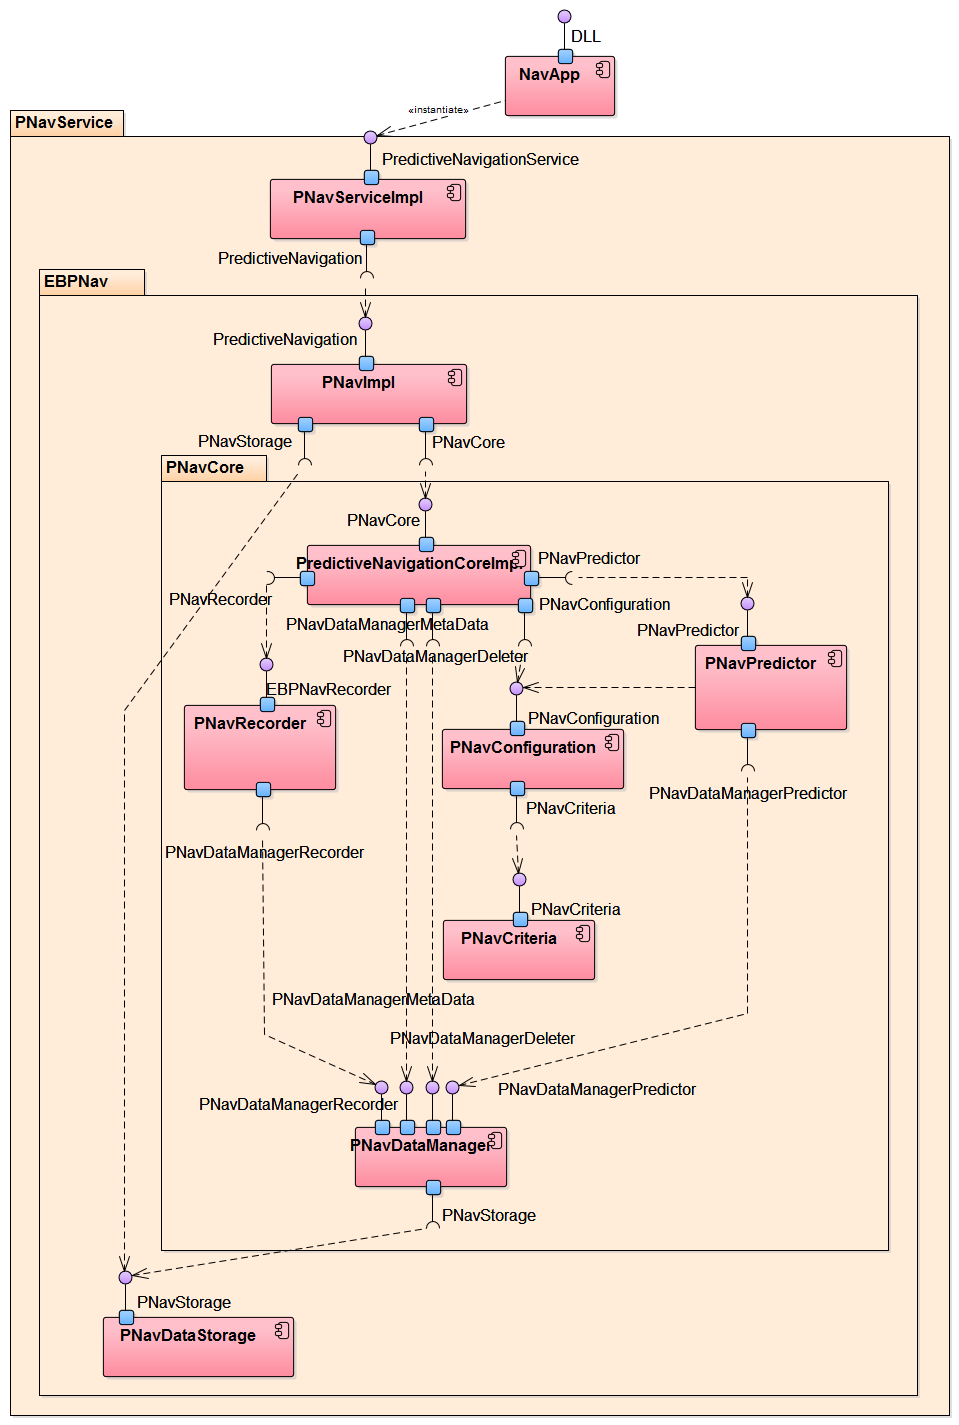
\includegraphics[width=0.8\textwidth]{Figures/pnav.png}}
  \caption{Diagrama componentelor}
  \end{figure}	
  
\subsection{Unitatea software PNavDLL} 
Această unitate realizează "ambalarea" întregului modul sub forma unei biblioteci cu legare dinamică (\acrfull{dll}).

\subsection{Unitatea software PNavCoreImpl} 
Unitatea PNavCoreImpl are rol de dispecer, utilizând restul unităților pentru realizarea funcționalităților de bază. 

\subsection{Unitatea software PNavServiceImpl} 
Unitatea PNavServiceImpl implementează interfaţa sincronă şi asincronă, şi îi oferă totodată dezvoltatorului posibilitatea de a alege ce interfaţă doreşte să folosească.
\vspace{6pt}
\\Cea asincronă are avantajul de a decupla firele de execuţie şi de a permite rularea activităţilor în paralel, însă are şi dezavantajul necesităţii de implementare unui mecanism de sincronizare în codul aplicaţiei în care va fi folosit modulul.


\subsection{Unitatea software PNavImpl} 
Deşi funcţionalităţile de bază precum precum învăţarea şi predicţia sunt realizare de către unitatea PNavRecorder respectiv PNavPredictor, unitatea PNavImpl realizează funcţionalităţi suplimentare cum ar fi multiple profile de utilizatori, ştergerea bazelor de date.
\vspace{6pt}
\\Funcţionalitatea multiplelor profile de utilizatori permite gestionarea mai multor baze de date, ce pot fi selectate pe baza unui ID de profil.
Acest ID poate cuprinde valori în intervalul 0-255. Pentru fiecare profil este creat un nou fişier în care vor fi stocate datele de utilizator. Unitatea PNavImpl implementează de asemenea şi funcţionalităţi de întreţinere a profilelor de utilizator precum ştergerea individuală, ştergerea totală, copierea, schimbarea între profile.

\subsection{Unitatea software PNavRecorder} 
NavRecorder-ul este unitate în care întreg procesul de învăţare are loc. 
\vspace{6pt}
\\Unitatea primeşte datele de geolocație şi de timp (oră - zi/lună/an) şi învaţă rutele parcurse de către dezvoltator într-un mod inteligent.
Acest lucru înseamnă că waypoint-urile (punctele prin care a trecut utilizatorul în timpul rutei sale) sunt stocate numai când autovehiculul şi-a schimbat 
orientarea semnificativ (valoare standard: > 15$^{\circ}$) sau distanţa dintre waypoint-uri nu este prea scurtă (valoare standard: > 200m). Valori pot fi configurate înaintea procesului de compilare.
\vspace{6pt}
\\Când sesiunea de înregistrare este finalizată, waypoint-urile sunt trimise către unitatea software PNavDataManager pentru a fi scrise în baza de date.
Totodată, unitatea are implementate funcţionalităţi de oprire-pornire, lucru ce-i acordă dezvoltatorului dreptul de opri şi porni oricând sesiunea de înregistrare.


\subsection{Unitatea software PNavPredictor} 
Rolul unităţii PNavPredictor este acela de a calcula predicţiile. 
\vspace{6pt}
\\Primul pas constă în încărcarea datelor prin unitatea PNavDataManager, care sunt mai departe prioritizate în funcţie de criterii specifice (descrise în tabela ~\ref{table:tabel_predictii}, ``Criterii de prioritizare pentru predicţia bazată pe rute''). Datele pot fi de asemenea filtrate pe baza aceloraşi criterii, rezultând astfel o cantitate mai mică de date şi un timp mai scurt de încărcare a acestora. 
\vspace{6pt}
\\Prioritizarea datelor este bazată atât pe datele de geolocație cât şi cele de timp, astfel încât o rută va avea o probabilitate mult mai mare de utilizare într-o anumită zi din săptămână sau la o anumită oră din zi.
\vspace{6pt}
\\Ca şi unitatea PNavRecorder, unitatea PNavPredictor are implementate funcţionalităţi de oprire-pornire.


\subsection{Unitatea software PNavConfiguration} 
Unitatea PNavConfiguration configurează unitatea NavPredictor, prin intermediul unor funcţii ce folosesc criteriile definite în unitatea PNavCriteria.


\subsection{Unitatea software PNavCriteria} 
Unitatea PNavCriteria conţine toate tipurile de criterii ce pot fi folosite la filtrarea sau prioritizarea datelor.
\vspace{6pt}
\\Fiecare criteriu în parte este folosit la procesarea datelor de către unitatea PNavPredictor.
După procesarea tuturor criteriilor cea mai probabilă rută este creată.


\subsection{Unitatea software PNavDataManager} 
Unitatea PNavDataManager implementează logica necesară pentru a realiza comunicarea între unitatea PNavDataStorage şi restul unităţilor.
\vspace{6pt}
\\În general, obiectele sunt stocate separat (e.g. rutele sunt stocate separat faţă de destinaţiilor lor). Cum însă pentru predicţia unei rute este nevoie de toate informaţiile, unitatea PNavDataManager le comasează. Aceasta oferă de asemenea şi alte funcţionalităţi precum adăugarea, gruparea, căutarea sau ştergerea de obiecte.


\subsection{Unitatea software PNavDataStorage} 
Unitatea PNavDataStorage este dezvoltată pe baza structurii bazei de date.
\vspace{6pt}
\\În afară de funcţionalitatea principală de a stoca sau încărca date, aceasta asigură şi accesarea selectivă a obiectelor. Pentru realizarea acestor funcţionalităţi se execută interogări prin intermediul SQLite.

% Chapter 1
\stepcounter{cap}
%\chapter{cap1}
\label{cap4}

\mychapter{4}{Capitolul \arabic{cap} \\ DESCRIEREA ALGORITMILOR}
%\chapter{\arabic{cap}.Introducere} % Main chapter title

\label{Chapter4} % For referencing the chapter elsewhere, use \ref{Chapter1} 

\thispagestyle{fancy}

%-----------------------------------------------------------------

\section{Învăţarea rutelor} 
Rutele sunt învăţate printr-un mecanism inteligent. Acest lucru are avantajul de a reduce semnificativ baza de date şi de a accelera încărcarea datelor.

	\subsection{Reducerea waypoint-urilor} 
	Criteriile pentru excluderea waypoint-urilor sunt:
	\begin{enumerate}
	 \setlength\itemsep{0em}
		\item Vehiculul nu şi-a schimbat orientarea semnificativ (valoare standard: > 15$^{\circ}$)
		\item Poziţiile sunt apropiate una de cealaltă (valoare standard: > 200m)
	\end{enumerate}
	
	Valorile standard pot fi configurate  înaintea procesului de compilare.
	
	
	\subsection{Verificarea rutelor duble} 
	
	\begin{figure}[h!]
   \centering
    \centering{%
      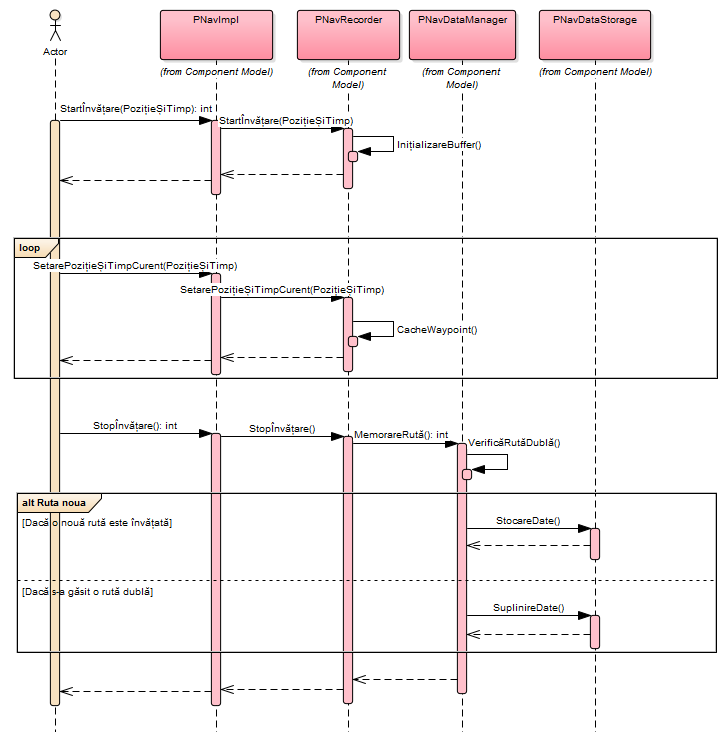
\includegraphics[width=0.9\textwidth]{Figures/rute_duble_sinc.png}}
   \caption{Procesul de verificarea al rutelor duble (sincron)}
   \end{figure}	
	
	În cazul în care ruta curentă are o secţiune similară cu o rută deja învăţată, unitatea software PNavDataManager va detecta secţiune respectivă şi va stoca numai waypoint-urile situate după aceasta. În schimb, toate destinaţiile sunt memorate. Criteriile pentru a detecta o astfel de rută sunt:
	
		\begin{enumerate}
	 \setlength\itemsep{0em}
		\item Destinaţia noii rute trebuie să fie situată într-o rază de 1km faţă de locaţia vechii destinaţii
		\item Punctul de start al noii rute trebuie să fie situată într-o rază de 1km faţă de punctul de plecare vechii destinaţii
		\item Toate waypoint-urile noii rute trebuie:
				\begin{enumerate}
				 \setlength\itemsep{0em}
					\item Să fie situat într-o anumită rază faţă de punctul de start al vechii rute
					\item Sau să fie situat într-o anumită rază faţă de destinaţia vechii rute
					\item Sau să fie situat într-o anumită rază faţă de un waypoint al vechii rute
				\end{enumerate}
	\end{enumerate}

Pragurile pot fi configurate înaintea procesului de compilare.


	\subsection{Filtrarea rutelor inutile}
	În timpul învăţării, rutele prea scurte (< 2km) nu vor fi stocate deoarece acest lucru ar însemna faptul că utilizatorul este destul de aproape de destinaţie.
	\vspace{6pt}
  \\Totodată, rutele foarte lungi (> 200km) vor fi de asemenea exclude din stocare deoarece ele nu reprezintă rute uzuale.
	\vspace{6pt}
  \\Pragurile pot fi configurate înaintea procesului de compilare.
	
\section{Eliberarea de spaţiu}   
Dacă pragul setat iniţial pentru dimensiunea maximă a bazei de date este atins, se va activa funcţia de eliberare a spaţiului. Aceasta va şterge obiectele cele mai vechi pentru a crea loc pentru obiectele noi.


	\begin{figure}[h!]
   \centering
    \centering{%
      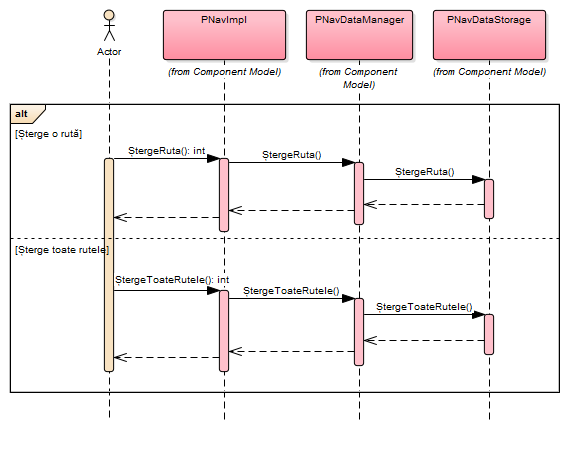
\includegraphics[width=0.9\textwidth]{Figures/sterge_ruta_sinc.png}}
   \caption{Procesul de ștergere a uneia sau mai multor rute (sincron)}
   \end{figure}	


\section{Furnizarea predicţiilor} 
Pentru ca predicţiile să fie disponibile sunt necesari doi paşi.
\vspace{6pt}
\\Primul pas reprezintă încărcarea datelor relevante, în timp de al doilea constă în prioritizarea lor.

	\begin{figure}[h!]
   \centering
    \centering{%
      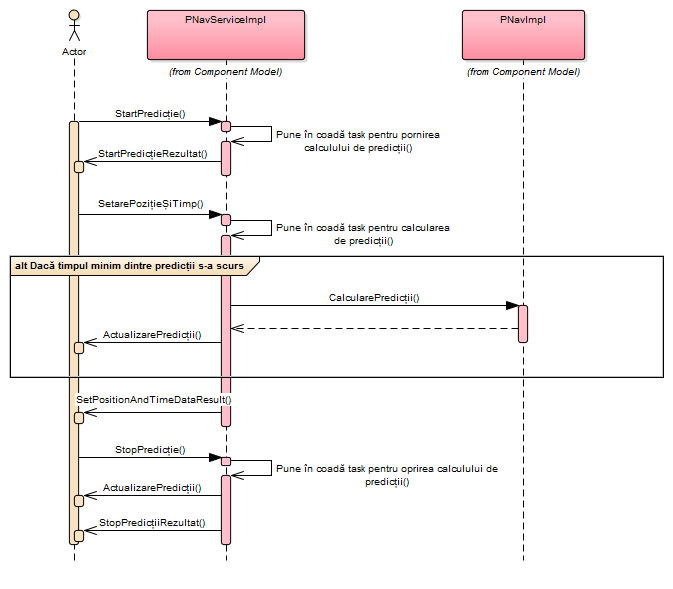
\includegraphics[width=0.9\textwidth]{Figures/calculare_predictii_asinc.png}}
   \caption{Procesul de calculare al predicțiilor(asincron)}
   \end{figure}	

	\subsection{Filtrarea datelor}
	Pentru o încărcare selectivă şi mai rapidă a datelor din unitatea PNavDataStorage, sunt create interogări. Sunt definiţi trei paşi în filtrare, unde pasul următor se excută doar în cazul în care cel curent nu a returnat destule rezultate:
		\begin{enumerate}
				 \setlength\itemsep{0em}
					\item Filtrarea rutei în funcţie de distanţa de la poziţia curentă la waypoint-urile rutelor
					\item Filtrarea rutei în funcţie de distanţa de la poziţia curentă la punctele de start ale rutelor
					\item Filtrarea rutelor în funcţie de timpul scurs până la ajungerea la destinaţie
		\end{enumerate}

	Toate rutele ce duc la o destinaţie situată la o distanţă mai mică de 1km faţă de poziţia actuală sunt ignorate deoarece utilizatorul aproape a ajuns la eventuala destinaţie.
	\vspace{6pt}
	\\În cazul predicţiilor baza pe timp, modulul furnizează o predicţie fără a cunoaşte ruta, ci doar destinaţia sa. Un astfel de caz ar fi cel în care utilizatorul a condus pe o rută în intervalul luni-miercuri, însă in ziua de joi a pornit de la o altă locaţie. Astfel, bazat pe timp, modulul prezice destinaţia fără a şti ruta corespunzătoare acesteia.
	
	
		\subsection{Frecvenţa predicţiei de rute}
		De obicei, waypoint-urile furnizate de modul de predicţie sunt transformate într-o rută ce foloseşte drumuri din hartă, fapt ce durează câteva secunde.
		Pentru a nu supraîncărca sistemul de navigaţie cu prea multe predicţii, dezvoltatorul poate seta timpul minim dintre două predicţii. Acestă setare se poate efectua chiar în timpul rulării.
		
		\subsection{Numărul maxim de predicţii}
		Pentru a putea suporta multiple platforme, modulul permite setarea numărului maxim de rute prezise ce apar deodată. Acestă setare se poate efectua chiar în timpul rulării.
		
		\subsection{Prioritizarea predicţiilor}
		Prioritatea unei rute reprezintă de fapt de probabilitatea ca această rută să fie ce pe care utilizatorul ar fi ales-o în mod uzual. Aceasta este exprimată sub formă de procente și se încadrează în intervalul 0\%-100\%.
		\vspace{6pt}
		\\Există mai multe criterii pentru a stabili prioritatea unei rute, fiecare dintre acestea fiind raportat la intervalul 0 (minimul) - 100 (maximul).  
		\vspace{6pt}
	    \\Pentru calcularea probabilității unei rute sunt necesari trei pași: 
	    
	    \begin{enumerate}
	     \setlength\itemsep{0em}
		 \item Pentru fiecare criteriu, se înmulțește ponderea cu probabilitatea sa 
		 \begin{equation}\label{qoat1}
		  SC = \sum_{i=1}^{n} p_{i}*c_{i}
		 \end{equation}
	     \item Se însumează toate criteriile  
		  \begin{equation}\label{qoat2}	      
	       SP = \sum_{i=1}^{n} p_{i}
	      \end{equation}
	     \item În urma raportului dintre suma de la pasul 1 și suma de la pasul 2,se obține probabilitatea rutei
	    \begin{equation}\label{qoat}	   
	     P = \frac{SC}{SP}
	    \end{equation}
    	\end{enumerate}
    	
		unde, \textit{P} = probabilitatea rutei, \textit{SC} = suma criteriilor, \textit{SP} = suma ponderilor, \textit{p} = ponderea criteriului, \textit{c} = probabilitatea criteriului (0\%-100\%), \textit{n} = numărul total de criterii	
		
		\vspace{6pt}
	    Metoda de definire a fiecărui criteriu depinde de criteriile însăși, după cum se observă în tabelele următoare.
		
		\begin{table}[!h]
		\caption{Criterii de prioritizare pentru predicţia bazată pe rute}
		\centering
		\begin{tabular}{ | m{2,7cm} | m{3,6cm} | m{3,22cm} | m{3,22cm} | m{1,4cm} | }
		\hline
		\textbf{Criteriu} & \textbf{Descriere} & \textbf{Min (0\% probabilitate)} & \textbf{Max (100\% probabilitate)} & \textbf{Pondere} \\ 
		\hline
		 Frecvenţa rutei & Numărul de utilizări al unei rute & Niciodată & Folosită de mai mult de 10 ori & 4 \\
		\hline
		 Frecvenţa rutei într-un anumit interval de timp & Numărul de utilizări al unei rute într-un anumit interval de timp (de la -1 oră la +2 ore) faţă de ora curentă & Niciodată & Folosită de mai mult de 10 ori & 1 \\
		\hline
		 Frecvenţa rutei într-o anumită zi & Numărul de utilizări al unei rute în ziua curentă din săptămână & Niciodată & Folosită de mai mult de 10 ori & 1 \\
		\hline
		 Frecvenţa rutei într-un anumit grup de zile & Numărul de utilizări al unei rute într-un anumit grup de zile (e.g. luni-vineri)& Niciodată &  Folosită de mai mult de 10 ori  & 1 \\
		\hline
		 Ultima utilizare a unei rute & Diferenţa dintre ultima utilizare a rutei şi ora/data curentă & >4 săptămâni & <2zile & 3 \\
		\hline
		 Distanţa până la destinaţie & Distanţa dintre poziţia actuală şi destinaţie & >100km & 0km & 1 \\
		\hline
		\end{tabular}
		\label{table:tabel_predictii}
		\end{table}
		
		
		\subsection{Predicţii bazate pe filtrarea rutei în funcţie de distanţa de la poziţia curentă la waypoint-urile rutelor}
		Criteriile definite în tabela ~\ref{table:tabel_predictii}, ``Criterii de prioritizare pentru predicţia bazată pe rute'' sunt extinse prin adăugarea următoarelor criterii:
		
		\begin{table}[!h]
		\caption{Criterii de prioritizare pentru predicţia bazată pe rutele din jurul unei poziţii}
		\centering
		\begin{tabular}{ | m{2,7cm} | m{3,6cm} | m{3,22cm} | m{3,22cm} | m{1,4cm} | }
		\hline
		\textbf{Criteriu} & \textbf{Descriere} & \textbf{Min (0\% probabilitate)} & \textbf{Max (100\% probabilitate)} & \textbf{Pondere} \\ 
		\hline
		 Distanţa până la rută & Distanţa dintre poziţia actuală şi waypoint-urile rutei &> 1km & 0km & 1 \\
		\hline
		 Direcţia către rută & Diferenţa dintre orientarea waypoint-urilor şi direcţia de navigare & 180$^{\circ}$ & 0$^{\circ}$ & 1 \\
		\hline
		\end{tabular}
		\end{table}
		
		
		\subsection{Predicţii bazate pe filtrarea rutei în funcţie de distanţa de la poziţia curentă la punctele de start ale rutelor}
		Criteriile definite în tabela ~\ref{table:tabel_predictii}, ``Criterii de prioritizare pentru predicţia bazată pe rute'' sunt extinse prin adăugarea următoarelor criterii:
		
		\begin{table}[!h]
		\caption{Criterii de prioritizare pentru predicţia bazată pe filtrarea rutele în funcţie de distanţa până la punctul de start al rutei}
		\centering
		\begin{tabular}{ | m{2,7cm} | m{3,6cm} | m{3,22cm} | m{3,22cm} | m{1,4cm} | }
		\hline
		\textbf{Criteriu} & \textbf{Descriere} & \textbf{Min (0\% probabilitate)} & \textbf{Max (100\% probabilitate)} & \textbf{Pondere} \\ 
		\hline
		 Distanţa până la punctul de start al rutei & Distanţa până la cel mai apropiat punct de start al rutei &> 3km & 0km & 1 \\
		\hline
		\end{tabular}
		\end{table}
		
		\subsection{Predicţii bazate pe filtrarea rutei în funcţie de timpul scurs până la ajungerea la destinaţie}
		Pentru acest caz sunt folosite criteriile definite în tabela ~\ref{table:tabel_predictii}, ``Criterii de prioritizare pentru predicţia bazată pe rute''.
		
		
		
		


	 
% Chapter 1
\stepcounter{cap}
%\chapter{cap1}
\label{cap5}

\mychapter{5}{Capitolul \arabic{cap} \\ MANAGEMENTUL ERORILOR}
%\chapter{\arabic{cap}.Introducere} % Main chapter title

\label{Chapter5} % For referencing the chapter elsewhere, use \ref{Chapter1} 

\thispagestyle{fancy}

%-----------------------------------------------------------------

\section{Tipuri de erori} 
\begin{itemize}
 \setlength\itemsep{0em}
	\item Erori de secvenţă
	\item Erori apărute la accesarea bazei de date
	\item Bază de date coruptă
\end{itemize}


\section{Detectarea erorilor}
Erorile sunt raportate pentru fiecare apel către şi dinspre interfaţa modului de predicţie. Toate funcţiile returnează un număr ce corespunde unui tip de eroare.

	\subsection{Erori de secvenţă}
	O maşină de stare va verifica încălcarea ordinii secvenţelor.
	
	\subsection{Erori la accesarea bazei de date}
	Trebuie evaluate rezultatele funcţiilor native de accesare ale bazei de date.

	\subsection{Bază de date coruptă}
	Trebuie evaluate rezultatele funcţiilor native de accesare ale bazei de date.
	
	
\section{Tratarea erorilor}
În funcţie de tipul de eroare, aceasta poate fi prevenită pe viitor sau nu de către dezvoltator.
\vspace{6pt}
\\Există erori de secvenţă precum ``Înainte de apelarea funcţiei X este necesară pornirea unităţii software PNavPredictor''. Se poate întâmpla de asemenea ca atunci când dezvoltatorul porneşte procesul de predicţie de două ori consecutiv sa fie întâmpinat de eroarea ``Procesul de predicţie se află deja în curs de rulare''.
În astfel de cazuri este clar cum se pot preveni erorile.
\vspace{6pt}
\\Mai sunt însă şi cazuri ce nu pot fi tratate de către dezvoltator. Astfel de erori sunt cele precum ``Baza de date este coruptă'', ce pot să apară în cazul în care fişierul de sistem folosit pentru stocarea datelor este corupt. În aceste situaţii datele stocate anterior nu mai pot fi recuperate, toate informaţiile referitoare la rute fiind definitiv pierdute.



 
% Chapter 1
\stepcounter{cap}
%\chapter{cap1}
\label{cap6}

\mychapter{6}{Capitolul \arabic{cap} \\ CONCLUZII ȘI DIRECȚII VIITOARE}
%\chapter{\arabic{cap}.Introducere} % Main chapter title

\label{Chapter6} % For referencing the chapter elsewhere, use \ref{Chapter1} 

\thispagestyle{fancy}

%-----------------------------------------------------------------

\section{Concluzii generale} 

\section{Posibilități de dezvoltare ulterioară} 
 



\end{document}  